\begin{explanationbox}
\textbf{一、先区分两个记号。}
\[\lfloor x\rfloor=\text{整数部分},\qquad \{x\}=x-\lfloor x\rfloor=\text{小数部分}.\]
例如 $x=2.7$ 时，$\lfloor x\rfloor=2$，$\{x\}=0.7$；当 $x=-2.3$ 时，$\lfloor x\rfloor=-3$，$\{x\}=0.7$。

\textbf{二、整数部分为什么叫“向下取整”？}
\[\begin{array}{c|rrrrrr}x&-2.3&-2&-0.1&0&1.9&2\\\hline \lfloor x\rfloor&-3&-2&-1&0&1&2\end{array}\]
向下是沿数轴向左，不是去掉小数点后的数字。
\begin{center}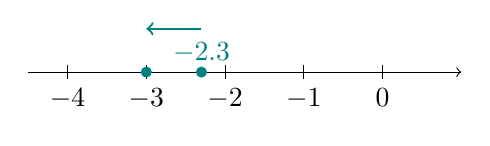
\begin{tikzpicture}\draw[->](-4.5,0)--(1,0);\foreach \n in {-4,-3,-2,-1,0}{\draw(\n,.09)--(\n,-.09) node[below]{$\n$};}\fill[teal](-2.3,0) circle(2pt) node[above]{$-2.3$};\draw[->,teal,thick](-2.3,.55)--(-3,.55);\fill[teal](-3,0) circle(2pt);\end{tikzpicture}\end{center}
在每个区间 $[n,n+1)$ 上，函数值恒等于 $n$，所以图像是一段一段的台阶。

\textbf{三、小数部分为什么总在 $[0,1)$ 内？}
设 $\lfloor x\rfloor=n$，则 $n\le x<n+1$。三边同减 $n$，得到
\[0\le x-n<1.\]
而 $x-n=x-\lfloor x\rfloor=\{x\}$，所以 $0\le\{x\}<1$。小数部分记录“从左侧整数出发已经走过多少”。横坐标每增加 $1$，所在区间与整数部分同时增加 $1$，剩余量不变，故 $\{x+1\}=\{x\}$。

\textbf{四、从图像过渡到不等式。} 例如 $\lfloor x\rfloor\le2$ 表示只允许高度不超过 $2$ 的台阶；最后一个允许的台阶是 $[2,3)$，因此全部允许的横坐标为 $x<3$。若 $\lfloor x\rfloor\ge2$，则从台阶 $[2,3)$ 开始向右全部允许，因此 $x\ge2$。这就是整数边界转换的几何意义。

\textbf{五、为什么加法有时会多出一个整数？} 把 $2.7=2+0.7$、$3.6=3+0.6$ 分开看。整数部分相加为 $5$，小数部分相加为 $1.3$，又贡献一个整数，故 $\lfloor2.7+3.6\rfloor=6$。
\begin{center}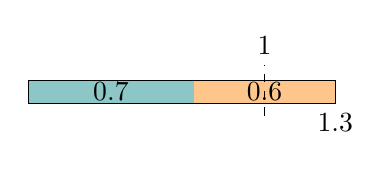
\begin{tikzpicture}[x=3cm]\fill[teal!45](0,0) rectangle(.7,.3);\fill[orange!45](.7,0) rectangle(1.3,.3);\draw(0,0) rectangle(1.3,.3);\draw[dashed](1,-.15)--(1,.5) node[above]{$1$};\node at (.35,.15){$0.7$};\node at (1,.15){$0.6$};\node[below] at (1.3,0){$1.3$};\end{tikzpicture}\end{center}

\textbf{六、识别方法。} 看到取整等式，立刻改写为左闭右开的区间；看到整数平移，先把整数移到符号外；看到加法，先检查小数部分之和是否达到 $1$。
\end{explanationbox}
